
%============================================================
\begin{frame}{Signal generators}{Numbers}
    %============================================================
    \begin{columns}
    \begin{column}{5cm}
    \begin{center}

    \lstinline'process = 1;'

    \vspace{0.5cm}

    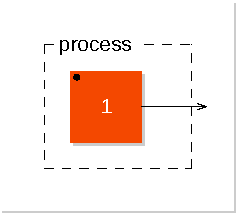
\includegraphics[scale=0.75]{images/un-process}

    \end{center}
    \end{column}

    \begin{column}{7cm}
    \begin{center}
    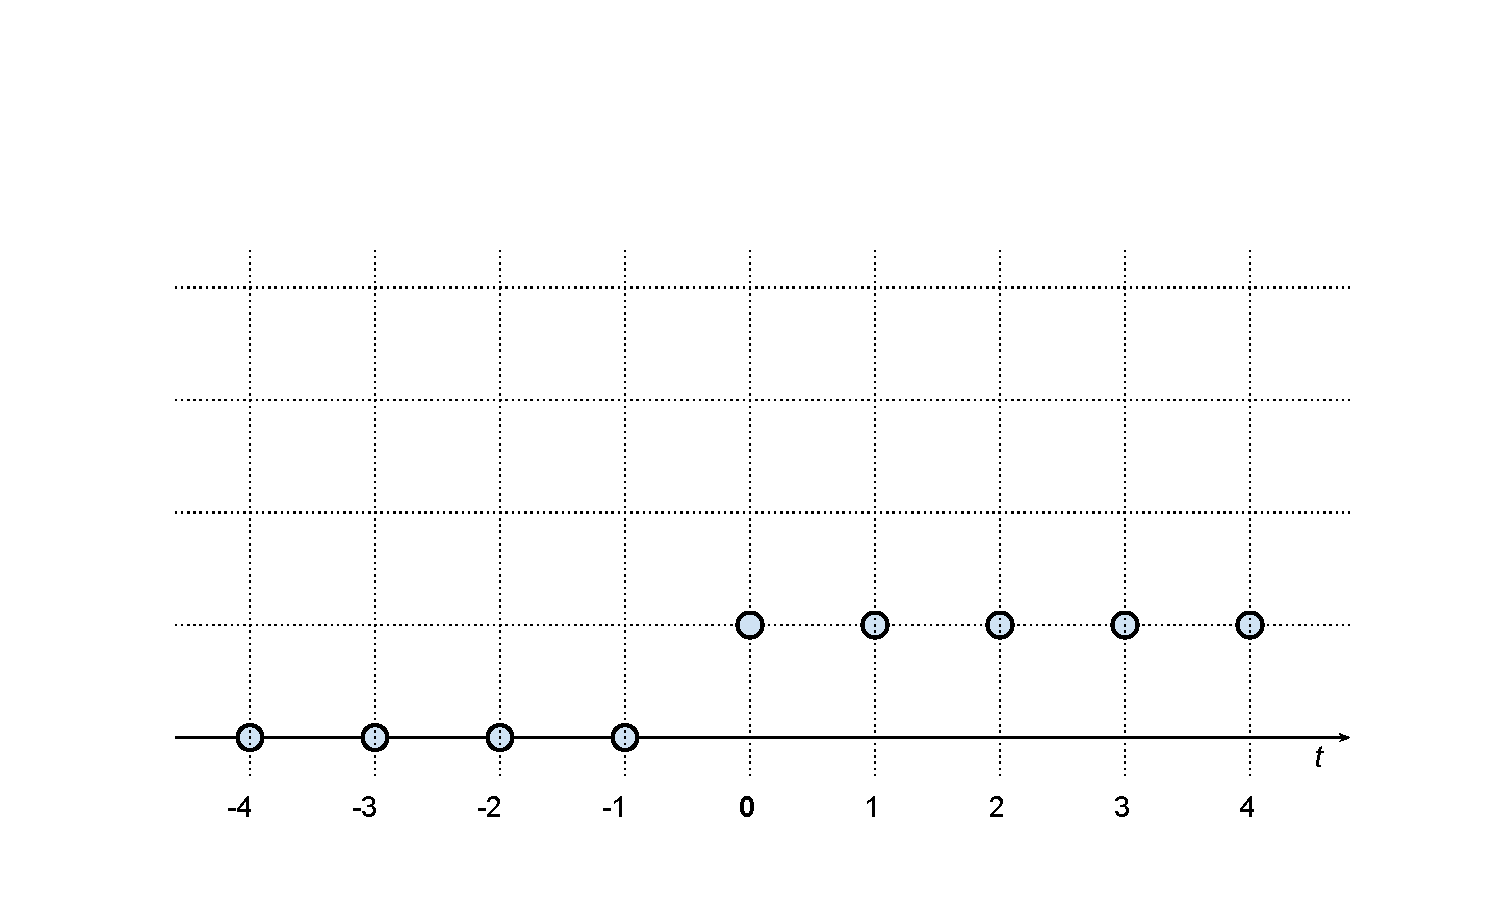
\includegraphics[width=7cm]{images/Faust-signal-1}

    %%% $x(t)=0$ when $t<0$ \\$x(t)=1$ when $t\geq 0$.

     \[
     y(t)=\left \{
             \begin{array}{l c l}
                 1  &  & t\geq 0\\
                 0  &  & t<0
             \end{array}
         \right .
     \]

    \end{center}
    \end{column}
    \end{columns}

\end{frame}


%============================================================
\begin{frame}{Signal generators}{UI widgets}
    %============================================================
    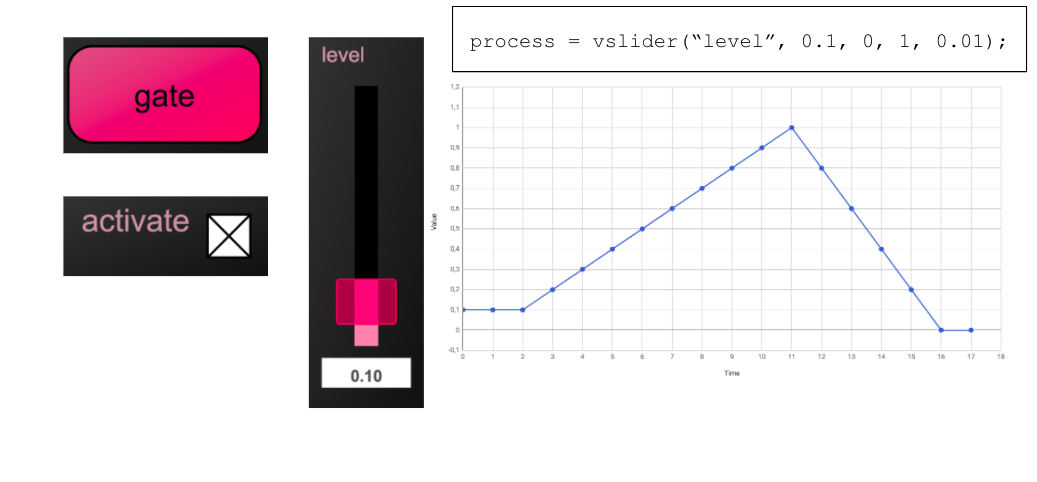
\includegraphics[width=1\textwidth]{images/ui}
\end{frame}

\begin{frame}[shrink=15, fragile]{Faust Primitives}
    \framesubtitle{Wire and Cut}
    \vspace{1cm}
    \begin{tabular}{|l|l|l|}
    \hline
    \textbf{Syntax} & \textbf{Type}  & \textbf{Description} \\
    \hline
    \lstinline|_| & $\mathbb{S}^{1}\rightarrow\mathbb{S}^{1}$ & wire: $y(t)=x(t)$ \\
    \lstinline|!| & $\mathbb{S}^{1}\rightarrow\mathbb{S}^{0}$ & cut: $<>, x(t) is ignored$ \\
    \hline
    \end{tabular}

    \end{frame}

\begin{frame}[shrink=15, fragile]{Faust Primitives}
    \framesubtitle{Arithmetic operations}
    \vspace{1cm}
    \begin{tabular}{|l|l|l|}
        \hline
        \textbf{Syntax} & \textbf{Type}  & \textbf{Description} \\
        \hline
        \texttt{+} & $\mathbb{S}^{2}\rightarrow\mathbb{S}^{1}$ & addition: $y(t)=x_{1}(t)+x_{2}(t)$  \\
        \texttt{-} & $\mathbb{S}^{2}\rightarrow\mathbb{S}^{1}$ & subtraction: $y(t)=x_{1}(t)-x_{2}(t)$   \\
        \texttt{*} & $\mathbb{S}^{2}\rightarrow\mathbb{S}^{1}$ & multiplication: $y(t)=x_{1}(t)*x_{2}(t)$   \\
        \texttt{$\land$} & $\mathbb{S}^{2}\rightarrow\mathbb{S}^{1}$ & power: $y(t)=x_{1}(t)^{x_{2}(t)}$   \\
        \texttt{/} & $\mathbb{S}^{2}\rightarrow\mathbb{S}^{1}$ & division: $y(t)=x_{1}(t)/x_{2}(t)$   \\
        \texttt{\%} & $\mathbb{S}^{2}\rightarrow\mathbb{S}^{1}$ & modulo: $y(t)=x_{1}(t)\%x_{2}(t)$   \\

        \texttt{int} & $\mathbb{S}^{1}\rightarrow\mathbb{S}^{1}$ & cast into an int signal: $y(t)=(int)x(t)$  \\
        \texttt{float} & $\mathbb{S}^{1}\rightarrow\mathbb{S}^{1}$ & cast into an float signal: $y(t)=(float)x(t)$  \\
        \hline

    \end{tabular}

\end{frame}


\begin{frame}[shrink=15, fragile]{Faust Primitives}
\framesubtitle{Bitwise operations}
\vspace{1cm}
\begin{tabular}{|l|l|l|}
\hline
\textbf{Syntax} & \textbf{Type}  & \textbf{Description} \\
\hline

\texttt{\&} & $\mathbb{S}^{2}\rightarrow\mathbb{S}^{1}$ & logical AND: $y(t)=x_{1}(t)\&x_{2}(t)$   \\
\texttt{|} & $\mathbb{S}^{2}\rightarrow\mathbb{S}^{1}$ & logical OR: $y(t)=x_{1}(t)|x_{2}(t)$   \\
\texttt{xor} & $\mathbb{S}^{2}\rightarrow\mathbb{S}^{1}$ & logical XOR: $y(t)=x_{1}(t)\land x_{2}(t)$   \\

\texttt{<<} & $\mathbb{S}^{2}\rightarrow\mathbb{S}^{1}$ & arith. shift left: $y(t)=x_{1}(t) << x_{2}(t)$   \\
\texttt{>>} & $\mathbb{S}^{2}\rightarrow\mathbb{S}^{1}$ & arith. shift right: $y(t)=x_{1}(t) >> x_{2}(t)$   \\

\hline

\end{tabular}

\end{frame}


\begin{frame}[shrink=15, fragile]{Faust Primitives}
\framesubtitle{Comparison operations}
\vspace{1cm}
\begin{tabular}{|l|l|l|}
\hline
\textbf{Syntax} & \textbf{Type}  & \textbf{Description} \\
\hline

\texttt{<} & $\mathbb{S}^{2}\rightarrow\mathbb{S}^{1}$ & less than: $y(t)=x_{1}(t) < x_{2}(t)$   \\
\texttt{<=} & $\mathbb{S}^{2}\rightarrow\mathbb{S}^{1}$ & less or equal: $y(t)=x_{1}(t) <= x_{2}(t)$   \\
\texttt{>} & $\mathbb{S}^{2}\rightarrow\mathbb{S}^{1}$ & greater than: $y(t)=x_{1}(t) > x_{2}(t)$   \\
\texttt{>=} & $\mathbb{S}^{2}\rightarrow\mathbb{S}^{1}$ & greater or equal: $y(t)=x_{1}(t) >= x_{2}(t)$   \\
\texttt{==} & $\mathbb{S}^{2}\rightarrow\mathbb{S}^{1}$ & equal: $y(t)=x_{1}(t) == x_{2}(t)$   \\
\texttt{!=} & $\mathbb{S}^{2}\rightarrow\mathbb{S}^{1}$ & different: $y(t)=x_{1}(t) != x_{2}(t)$   \\

\hline

\end{tabular}

\end{frame}


\begin{frame}[shrink=15, fragile]{Faust Primitives}
\framesubtitle{Trigonometric functions}
\vspace{1cm}
\begin{tabular}{|l|l|l|}
\hline
\textbf{Syntax} & \textbf{Type}  & \textbf{Description} \\
\hline
\texttt{acos} & $\mathbb{S}^{1}\rightarrow\mathbb{S}^{1}$ & arc cosine: $y(t)=\mathrm{acosf}(x(t))$ \\
\texttt{asin} & $\mathbb{S}^{1}\rightarrow\mathbb{S}^{1}$ & arc sine: $y(t)=\mathrm{asinf}(x(t))$ \\
\texttt{atan} & $\mathbb{S}^{1}\rightarrow\mathbb{S}^{1}$ & arc tangent: $y(t)=\mathrm{atanf}(x(t))$ \\
\texttt{atan2} & $\mathbb{S}^{2}\rightarrow\mathbb{S}^{1}$ & arc tangent of 2 signals: $y(t)=\mathrm{atan2f}(x_{1}(t), x_{2}(t))$ \\

\texttt{cos} & $\mathbb{S}^{1}\rightarrow\mathbb{S}^{1}$ & cosine: $y(t)=\mathrm{cosf}(x(t))$ \\
\texttt{sin} & $\mathbb{S}^{1}\rightarrow\mathbb{S}^{1}$ & sine: $y(t)=\mathrm{sinf}(x(t))$ \\
\texttt{tan} & $\mathbb{S}^{1}\rightarrow\mathbb{S}^{1}$ & tangent: $y(t)=\mathrm{tanf}(x(t))$ \\
\hline
\end{tabular}

\end{frame}



\begin{frame}[shrink=15, fragile]{Faust Primitives}
\framesubtitle{Other Math operations}
\vspace{1cm}
\begin{tabular}{|l|l|l|}
\hline
\textbf{Syntax} & \textbf{Type}  & \textbf{Description} \\
\hline

\texttt{exp} & $\mathbb{S}^{1}\rightarrow\mathbb{S}^{1}$ & base-e exponential: $y(t)=\mathrm{expf}(x(t))$ \\
\texttt{log} & $\mathbb{S}^{1}\rightarrow\mathbb{S}^{1}$ & base-e logarithm: $y(t)=\mathrm{logf}(x(t))$ \\
\texttt{log10} & $\mathbb{S}^{1}\rightarrow\mathbb{S}^{1}$ & base-10 logarithm: $y(t)=\mathrm{log10f}(x(t))$ \\
\texttt{pow} & $\mathbb{S}^{2}\rightarrow\mathbb{S}^{1}$ & power: $y(t)=\mathrm{powf}(x_{1}(t),x_{2}(t))$ \\
\texttt{sqrt} & $\mathbb{S}^{1}\rightarrow\mathbb{S}^{1}$ & square root: $y(t)=\mathrm{sqrtf}(x(t))$ \\
\texttt{abs} & $\mathbb{S}^{1}\rightarrow\mathbb{S}^{1}$ & absolute value (int): $y(t)=\mathrm{abs}(x(t))$ \\
			&											 & absolute value (float): $y(t)=\mathrm{fabsf}(x(t))$ \\
\texttt{min} & $\mathbb{S}^{2}\rightarrow\mathbb{S}^{1}$ & minimum: $y(t)=\mathrm{min}(x_{1}(t),x_{2}(t))$ \\
\texttt{max} & $\mathbb{S}^{2}\rightarrow\mathbb{S}^{1}$ & maximum: $y(t)=\mathrm{max}(x_{1}(t),x_{2}(t))$ \\
\texttt{fmod} & $\mathbb{S}^{2}\rightarrow\mathbb{S}^{1}$ & float modulo: $y(t)=\mathrm{fmodf}(x_{1}(t),x_{2}(t))$ \\
\texttt{remainder} & $\mathbb{S}^{2}\rightarrow\mathbb{S}^{1}$ & float remainder: $y(t)=\mathrm{remainderf}(x_{1}(t),x_{2}(t))$ \\

\texttt{floor} & $\mathbb{S}^{1}\rightarrow\mathbb{S}^{1}$ & largest int $\leq$: $y(t)=\mathrm{floorf}(x(t))$ \\
\texttt{ceil} & $\mathbb{S}^{1}\rightarrow\mathbb{S}^{1}$ & smallest int $\geq$: $y(t)=\mathrm{ceilf}(x(t))$ \\
\texttt{rint} & $\mathbb{S}^{1}\rightarrow\mathbb{S}^{1}$ & closest int: $y(t)=\mathrm{rintf}(x(t))$ \\

\hline
\end{tabular}
\end{frame}


%%%%%%%%%% Expressions %%%%%%%%%%%%%%%%%%
%\begin{frame}[shrink=15, fragile]{Faust Primitives}
%\framesubtitle{Add new ones using Foreign Functions}
%
%\begin{rail}
%foreignexp : 'ffunction' '(' signature ',' inclfile ',' comment ')'
%          | 'fvariable' '(' type identifier ',' inclfile ')'
%          | 'fconstant' '(' type identifier ',' inclfile ')' ;
%\end{rail}
%
%\begin{itemize}
%\item Reference to external C \textit{functions}, \textit{variables} and \textit{constants} can be introduced using the \textit{foreign function} mechanism.
%
%\item example :
%\begin{lstlisting}
%asinh = ffunction(float asinhf (float), <math.h>, "");
%\end{lstlisting}
%
%
%\end{itemize}
%\end{frame}



%%%%%%%%%%%%%%%%%%%%%%%%%%%%%%%%%%%%%%%%%%%%%%%%%%%%%%%%%%%%%%%%%%%%%%%%

\begin{frame}[shrink=15, fragile]{Faust Primitives}
\framesubtitle{Delays and Tables}
\vspace{1cm}
\begin{tabular}{|l|l|l|}
\hline
\textbf{Syntax} & \textbf{Type}  & \textbf{Description} \\
\hline

\texttt{mem} & $\mathbb{S}^{1}\rightarrow\mathbb{S}^{1}$ 		& 1-sample delay: 	$y(t+1)=x(t),y(0)=0$  \\
%%%\texttt{prefix} & $\mathbb{S}^{2}\rightarrow\mathbb{S}^{1}$ 	& 1-sample delay:  	$y(t+1)=x_{2}(t),y(0)=x_{1}(0)$  \\
\texttt{@} & $\mathbb{S}^{2}\rightarrow\mathbb{S}^{1}$ 			& delay:  	$y(t+x_{2}(t))=x_{1}(t), y(t<x_{2}(t))=0$  \\

\texttt{rdtable} & $\mathbb{S}^{3}\rightarrow\mathbb{S}^{1}$ 	& read-only table:	$y(t)=T[r(t)]$  \\
\texttt{rwtable} & $\mathbb{S}^{5}\rightarrow\mathbb{S}^{1}$ 	& read-write table:	$T[w(t)]=c(t); y(t)=T[r(t)]$  \\

\texttt{select2} & $\mathbb{S}^{3}\rightarrow\mathbb{S}^{1}$ 	& between 2 sig:	$T[]=\{x_{0}(t),x_{1}(t)\}; y(t)=T[s(t)]$  \\
\texttt{select3} & $\mathbb{S}^{4}\rightarrow\mathbb{S}^{1}$ 	& between 3 sig:	$T[]=\{x_{0}(t),x_{1}(t),x_{2}(t)\}; y(t)=T[s(t)]$  \\

\hline
\end{tabular}

\end{frame}



%%%%%%%%%%%%%%%%%%%%%%%%%%%%%%%%%%%%%%%%%%%%%%%%%%%%%%%%%%%%%%%%%%%%%%%%

\begin{frame}[shrink=15, fragile]{Faust Primitives}
\framesubtitle{Other User Interface Primitives}
\vspace{1cm}
\begin{tabular}{|l|l|}
\hline
\textbf{Syntax} &  \textbf{Example} \\
\hline
\texttt{vgroup(\farg{str},\farg{block-diagram})} & \texttt{vgroup("reverb", \ldots)}\\
\texttt{hgroup(\farg{str},\farg{block-diagram})} & \texttt{hgroup("mixer", \ldots)}\\
\texttt{tgroup(\farg{str},\farg{block-diagram})} & \texttt{vgroup("parametric", \ldots)}\\
\texttt{vbargraph(\farg{str},\farg{min},\farg{max})} & \texttt{vbargraph("input",0,100)}\\
\texttt{hbargraph(\farg{str},\farg{min},\farg{max})} & \texttt{hbargraph("signal",0,1.0)}\\

\hline
\end{tabular}

\end{frame}


